% Working research-report draft. The supplied template remains unchanged in ../Template/.
\documentclass[journal,10pt,twoside]{IEEEtran}

\usepackage[utf8]{inputenc}
\usepackage[T1]{fontenc}
\usepackage{graphicx}
\usepackage{amsmath,amssymb,mathtools}
\usepackage{booktabs}
\usepackage{enumitem}
\usepackage{xcolor}
\usepackage{tikz}
\usetikzlibrary{positioning,arrows.meta,calc}
\usepackage{balance}
\usepackage{microtype}
\usepackage{dblfloatfix}
\usepackage{url}
\usepackage[bookmarks=true,bookmarksopen=true]{hyperref}
\usepackage{cleveref}
\usepackage{natbib}\input{natbib-add}
\bibliographystyle{apalike}
\bibpunct{[}{]}{;}{a}{}{}

\setlist[itemize]{noitemsep,nolistsep,leftmargin=*}
\setlist[enumerate]{noitemsep,nolistsep,leftmargin=*}
\hypersetup{colorlinks=true,urlcolor=blue,linkcolor=blue,citecolor=blue}
\crefname{figure}{figure}{figures}
\Crefname{figure}{Figure}{Figures}
\crefname{table}{table}{tables}
\Crefname{table}{Table}{Tables}

\newcommand{\reporttitle}{Spatial Context and Nonlinear Attribution for Peak Learning in Mass Spectrometry Imaging}
\newcommand{\authorname}{Zayd \textsc{Suliman}}
\newcommand{\studentnumber}{2653934}
\newcommand{\supervisorname}{Hairong Bau and Richard Klein}
\newcommand{\academicyear}{2026}

\begin{document}

\title{%
  \vspace{4pt}
  
\includegraphics[width=0.12\textwidth]{images/witslogonew.png}\\[6pt]
  \Large\textbf{\reporttitle}%
}

\author{%
  \authorname,~Student~No.~\studentnumber\\
  \small School of Computer Science and Applied Mathematics,
         Faculty of Science, University of the Witwatersrand\\
  \small Supervisors:~\supervisorname \qquad \academicyear
}

\maketitle

\begin{abstract}
Mass spectrometry imaging measures a high-dimensional mass spectrum at each
tissue location, making reliable feature reduction necessary before downstream
analysis. Existing variational-autoencoder peak learning is computationally
accessible but spatially blind, whereas spatial convolutional methods use local
structure at greater architectural complexity. This study separates two
possible sources of improvement: adding local neighbourhood context to a
lightweight variational autoencoder and replacing weight-based peak extraction
with nonlinear attribution. Centre-only and eight-neighbour contextual models
were trained under matched conditions on eight glioblastoma and eight
colorectal-adenocarcinoma sections. A label-free two-component Gaussian mixture
model was fitted to frozen latent means, and its posterior was attributed to
mass-to-charge bins using Integrated Gradients. At matched peak counts,
nonlinear attribution outperformed legacy msiPL on every section: mean mSCF1
increased from 0.3643 to 0.4562 on glioblastoma and from 0.4024 to 0.5595 on
colorectal adenocarcinoma. Uniform neighbourhood context was not universally
beneficial; it had no consistent glioblastoma advantage, but improved mSCF1
over the centre-only control on all eight colorectal sections. Corrected
attention improved mSCF1 over uniform averaging across three training seeds on
one development section, but did not improve deletion faithfulness and used
more memory. The principal result is therefore a robust gain from nonlinear,
label-free attribution, with spatial context providing a conditional rather
than universal benefit.
\end{abstract}

\begin{IEEEkeywords}
mass spectrometry imaging, peak learning, variational autoencoder, spatial context, Integrated Gradients, explainable artificial intelligence
\end{IEEEkeywords}

\section{Introduction}
\label{sec:introduction}

Mass spectrometry imaging (MSI) maps molecular measurements directly to tissue
coordinates, enabling biochemical structure to be studied without preselecting
one target molecule~\citep{caprioli1997maldi,schwamborn2010molecular}. Each
pixel nevertheless contains a spectrum with hundreds to tens of thousands of
mass-to-charge ($m/z$) bins. Many bins are redundant, noisy or unrelated to the
biological structure of interest, so selecting a compact set of informative
peaks is an important preprocessing step.

Conventional peak picking uses rules such as intensity and signal-to-noise
thresholds. These rules are useful but can be sensitive to user choices and may
discard weak yet spatially coherent ions. Peak learning instead trains a model
on spectra and derives a ranking from the learned representation. The msiPL
approach uses a one-dimensional variational autoencoder (VAE), but processes
each pixel independently~\citep{abdelmoula2021peak}. S3PL explicitly consumes a
spatial patch~\citep{weigand2026spatial}, although its three-dimensional
convolutional architecture and released implementation differ substantially
from msiPL. This leaves two questions entangled: whether local context improves
the learned representation, and whether a better explanation of a nonlinear
representation improves the resulting peak list.

This report develops Spatial-msiPL, a controlled VAE study in which the central
spectrum is compared with the same model supplied with a summary of its Moore
neighbourhood. Rather than assuming that first-layer weights faithfully explain
the model, a label-free Gaussian mixture model (GMM) is fitted in latent space
and its posterior is propagated to input bins with Integrated
Gradients~\citep{sundararajan2017axiomatic}. Expert masks are used only after
ranking to quantify spatial peak quality.

The study answers three research questions:
\begin{enumerate}
  \item Under matched training, how does eight-neighbour context affect
  reconstruction, latent tissue separation and matched-count peak quality
  relative to a centre-only VAE?
  \item Does nonlinear GMM-targeted Integrated Gradients produce better peak
  rankings than legacy msiPL and simple first-layer L2 importance?
  \item What peak-quality, explanation-faithfulness and computational trade-offs
  arise from learned attention, and are they stable across training seeds?
\end{enumerate}

The aim is to determine separately when neighbourhood context and nonlinear
attribution improve lightweight MSI peak learning. The principal contributions
are: (i) a controlled centre-only/contextual comparison; (ii) a label-free
GMM-targeted attribution pipeline; (iii) matched-count validation on eight GBM
and eight CAC sections; and (iv) completeness, deletion-faithfulness, compute
and training-seed analyses that bound the claims. The remainder of the report
reviews related peak-learning and attribution methods, defines the controlled
pipeline, presents the experimental results, and discusses what they do and do
not establish.

\section{Related Work}
\label{sec:related_work}

\subsection{MSI feature reduction}

MSI combines spectral and image structure, but its scale motivates feature
reduction before visualisation, classification or biological interpretation.
Traditional workflows include normalisation, smoothing, baseline correction
and rule-based peak detection~\citep{gibb2012maldiquant,deininger2011normalization}.
Sparse and learning-based methods reduce manual threshold dependence, but a
selected peak is useful for this study only when its ion image also reflects
annotated tissue structure~\citep{lieb2020sparse,winderbaum2015feature}.

\subsection{Representation and peak learning}

VAEs learn a probabilistic low-dimensional representation by balancing
reconstruction against regularisation of the latent distribution
~\citep{kingma2014autoencoding}. msiPL applies this idea to spectra and derives
peaks through network-weight analysis~\citep{abdelmoula2021peak}. Its small
network is attractive computationally, but neighbouring pixels do not interact.
S3PL introduces spatial self-supervision and patch-based convolutions, and also
provides a correlation-based evaluation that converts ion-image agreement with
tissue masks into mSCF1~\citep{weigand2026spatial}. These methods motivate a
lighter controlled test of spatial context inside an msiPL-style VAE.

\subsection{Neural attribution}

A first-layer weight norm measures only the model's initial linear connection
to each input. It cannot represent batch normalisation, nonlinear hidden
transformations, latent geometry or the downstream decision surface.
Integrated Gradients instead integrates the gradient of a chosen output along
a path from a baseline input to the observed input and satisfies a completeness
property under standard differentiability assumptions
~\citep{sundararajan2017axiomatic}. The present work targets a label-free GMM
posterior rather than a supervised class output. This lets attribution explain
which $m/z$ bins support structure learned without using expert tissue labels.

The project is therefore positioned as a controlled decomposition rather than
a claim that a new architecture dominates every baseline: the same VAE and
attribution procedure are used to isolate neighbourhood value, while matched
peak budgets isolate ranking quality.

\section{Methodology}
\label{sec:methodology}

\subsection{System overview}

\Cref{fig:pipeline} separates training, label-free explanation and mask-based
evaluation. No expert label is used to train the VAE, fit the GMM or produce the
peak ranking.

\begin{figure*}[t]
  \centering
  \resizebox{0.96\textwidth}{!}{%
  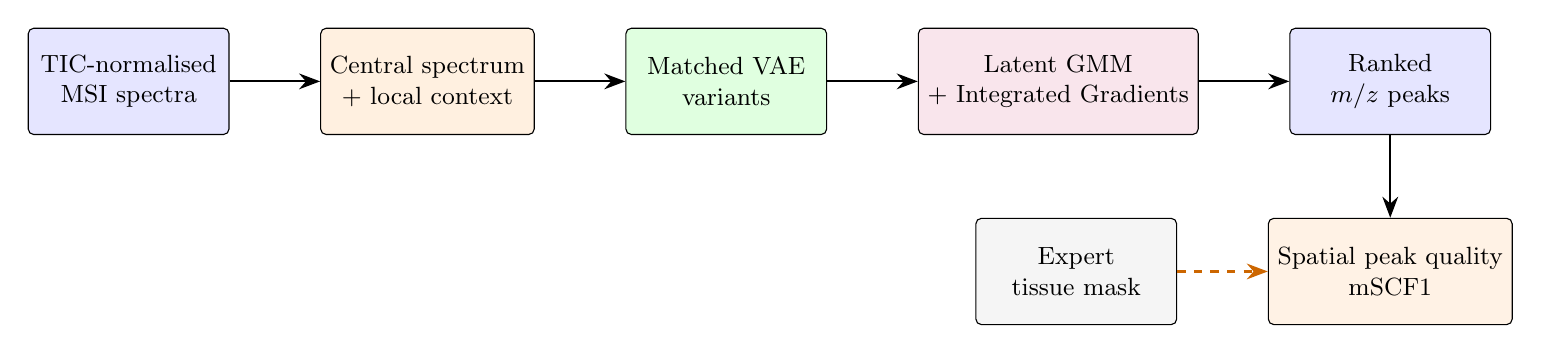
\begin{tikzpicture}[
    node distance=1.15cm,
    box/.style={draw, rectangle, rounded corners=2pt, minimum height=1.35cm,
      minimum width=2.55cm, align=center, font=\small, fill=gray!10},
    arrow/.style={-{Stealth[scale=1.15]}, thick},
    evalarrow/.style={-{Stealth[scale=1.15]}, thick, dashed, draw=orange!80!black}
  ]
    \node[box, fill=blue!10] (spectra) {TIC-normalised\\MSI spectra};
    \node[box, fill=orange!12, right=of spectra] (context) {Central spectrum\\$+$ local context};
    \node[box, fill=green!12, right=of context] (vae) {Matched VAE\\variants};
    \node[box, fill=purple!10, right=of vae] (explain) {Latent GMM\\$+$ Integrated Gradients};
    \node[box, fill=blue!10, right=of explain] (peaks) {Ranked\\$m/z$ peaks};
    \node[box, fill=orange!10, below=1.05cm of peaks] (score) {Spatial peak quality\\mSCF1};
    \node[box, fill=gray!8, left=1.15cm of score] (mask) {Expert\\tissue mask};

    \draw[arrow] (spectra) -- (context);
    \draw[arrow] (context) -- (vae);
    \draw[arrow] (vae) -- (explain);
    \draw[arrow] (explain) -- (peaks);
    \draw[arrow] (peaks) -- (score);
    \draw[evalarrow] (mask) -- (score);
  \end{tikzpicture}%
  }
  \caption{Simplified Spatial-msiPL workflow. Each measured spectrum is
  TIC-normalised and supplied either alone or with a summary of its valid
  eight-position Moore neighbourhood. Matched VAE variants reconstruct the
  central spectrum. After training, a label-free two-component GMM is fitted to
  frozen latent means and its posterior is attributed to the original $m/z$
  bins using Integrated Gradients. The resulting ranking is evaluated at a
  matched peak budget. The dashed path emphasises that expert tissue masks are
  used only to calculate mSCF1 after peak selection, never to train the VAE,
  fit the GMM or generate the ranking.}
  \label{fig:pipeline}
\end{figure*}

\subsection{Datasets and preprocessing}

Two public MSI collections were used (\Cref{tab:data}). The MassNet GBM data
contain eight sections with normal/tumour annotations and a shared 85,062-bin
axis~\citep{abdelmoula2022massnet}. Grid coverage ranges from 54.62\% to
82.95\%, so neighbourhoods are constructed from measured coordinates rather
than by treating missing grid locations as spectra. The CAC collection contains
eight sections, 1,481 bins and three mask classes. Seven grids are complete;
\texttt{280TopL} has 4,160 measured pixels in a 4,623-position grid (89.98\%
coverage). Coordinate--mask alignment and HDF5 round trips were audited before
training.

\begin{table}[t]
\caption{Dataset characteristics used by the experiments.}
\label{tab:data}
\centering
\begin{tabular}{lrrrl}
\toprule
Collection & Sections & Bins & Classes & Coverage \\
\midrule
GBM & 8 & 85,062 & 2 & 54.62--82.95\% \\
CAC & 8 & 1,481 & 3 & 89.98--100\% \\
\bottomrule
\end{tabular}
\end{table}

Each measured spectrum $s_i$ is total-ion-count (TIC) normalised,
\begin{equation}
x_i = \frac{s_i}{\sum_j s_{ij}+\epsilon},
\end{equation}
which reduces total-intensity scale differences while preserving relative bin
composition. The expert masks are retained separately for evaluation.

\subsection{Controlled VAE variants}

The centre-only control receives $x_i$. The uniform contextual model computes
the mean $c_i$ of the valid spectra in the eight-position Moore neighbourhood
and receives $[x_i,c_i]$. Missing neighbours contribute neither values nor
weights. The corrected-attention variant learns neighbour weights and applies
sqrt-bin input scaling before its scoring operation to avoid nearly uniform
scores caused by the small TIC-normalised magnitudes. All variants use a
512-unit hidden layer and a five-dimensional Gaussian latent representation.
The decoder reconstructs the central spectrum, so added context is useful only
if it helps explain the same target.

For a sample $x$, the objective is
\begin{equation}
\mathcal{L}=\mathcal{L}_{\mathrm{recon}}(x,\hat{x})+
\beta D_{\mathrm{KL}}\!\left(q_\phi(z\mid x,c)\|\mathcal{N}(0,I)\right).
\end{equation}
Matched comparisons use the same optimiser, schedule, split, epoch count and
seed. Production VAE runs use 100 epochs. Explicit adjacent-latent penalties
and Poisson augmentation were evaluated as development gates but were not
promoted: the former forced smoothness while degrading reconstruction, and the
latter did not reach its predeclared noisy-reconstruction improvement.

\subsection{Label-free nonlinear attribution}

After training, posterior means $\mu_i$ are frozen and a two-component GMM is
fitted without tissue labels. For pixel $i$, the scalar attribution target is
the posterior probability of its assigned component, $F_i=p(k_i\mid\mu_i)$.
For input $x$ and section-mean baseline $x'$, Integrated Gradients for bin $j$
is approximated by
\begin{equation}
\mathrm{IG}_j(x)=(x_j-x'_j)\frac{1}{M}
\sum_{m=1}^{M}\frac{\partial F(x'+\frac{m}{M}(x-x'))}{\partial x_j}.
\end{equation}
Absolute attributions are aggregated by $m/z$ across sampled pixels and GMM
components. Component-specific rankings are combined deterministically. For a
contextual model, contributions through the central and neighbourhood paths
are mapped to the same spectral bins before aggregation.

Completeness checks whether summed attributions approximate
$F(x)-F(x')$. Deletion faithfulness replaces highly ranked bins by baseline
values and measures the reduction in assigned-component posterior; a larger
drop indicates a more causally influential ranking. First-layer L2 importance
is retained as a deliberately simple linear comparator.

\subsection{Peak evaluation and statistical design}

For every $m/z$ bin, its ion image is correlated with each expert class mask
using Pearson's $r$. At a threshold $t\in\{0.3,0.4,0.5,0.6\}$, sufficiently
correlated bins form a reference-positive set. Precision and recall of a
selected peak list yield $F1_t$, and
\begin{equation}
\mathrm{mSCF1}=\frac{F1_{0.3}+F1_{0.4}+F1_{0.5}+F1_{0.6}}{4}.
\end{equation}
Within a section, compared methods select the same number of peaks. Results are
paired by section and exact two-sided Wilcoxon signed-rank tests are reported
where applicable. Section spread is not interpreted as patient-level
independence. Broad GBM and CAC validation uses seed 1; a targeted
GBM108-positive experiment repeats training with seeds 1--3 for centre-only,
uniform-mean and corrected-attention variants.

\section{Experiments and Results}
\label{sec:results}

\subsection{Baseline reproduction}

The tuned legacy msiPL reproduction obtained mean mSCF1 0.414 on GBM and 0.402
on CAC. These values lie inside the published aggregate intervals used for the
reproduction audit. S3PL was executable on both collections, but its GBM mean
remained below the reported paper result despite patch-size, normalisation,
format and mask checks. The CAC S3PL checkpoints were therefore re-evaluated at
the same section-specific peak counts as the VAE methods; no retraining was
needed. Matched S3PL averaged 0.5915 mSCF1.

\subsection{Does uniform context improve the VAE?}

On GBM, reconstruction MSE favoured uniform context in four sections and the
centre-only model in four (exact Wilcoxon $p=0.945$). Mean relative MSE change
was $-2.14\%$, but the median was $+0.52\%$ and one section strongly influenced
the mean. Uniform context used 130,751,056 parameters and approximately 2.90
GiB peak GPU memory, compared with 87,199,312 parameters and 2.05 GiB for the
centre-only model. \Cref{fig:recon} shows that local context did not provide a
consistent reconstruction advantage.

\begin{figure}[t]
  \centering
  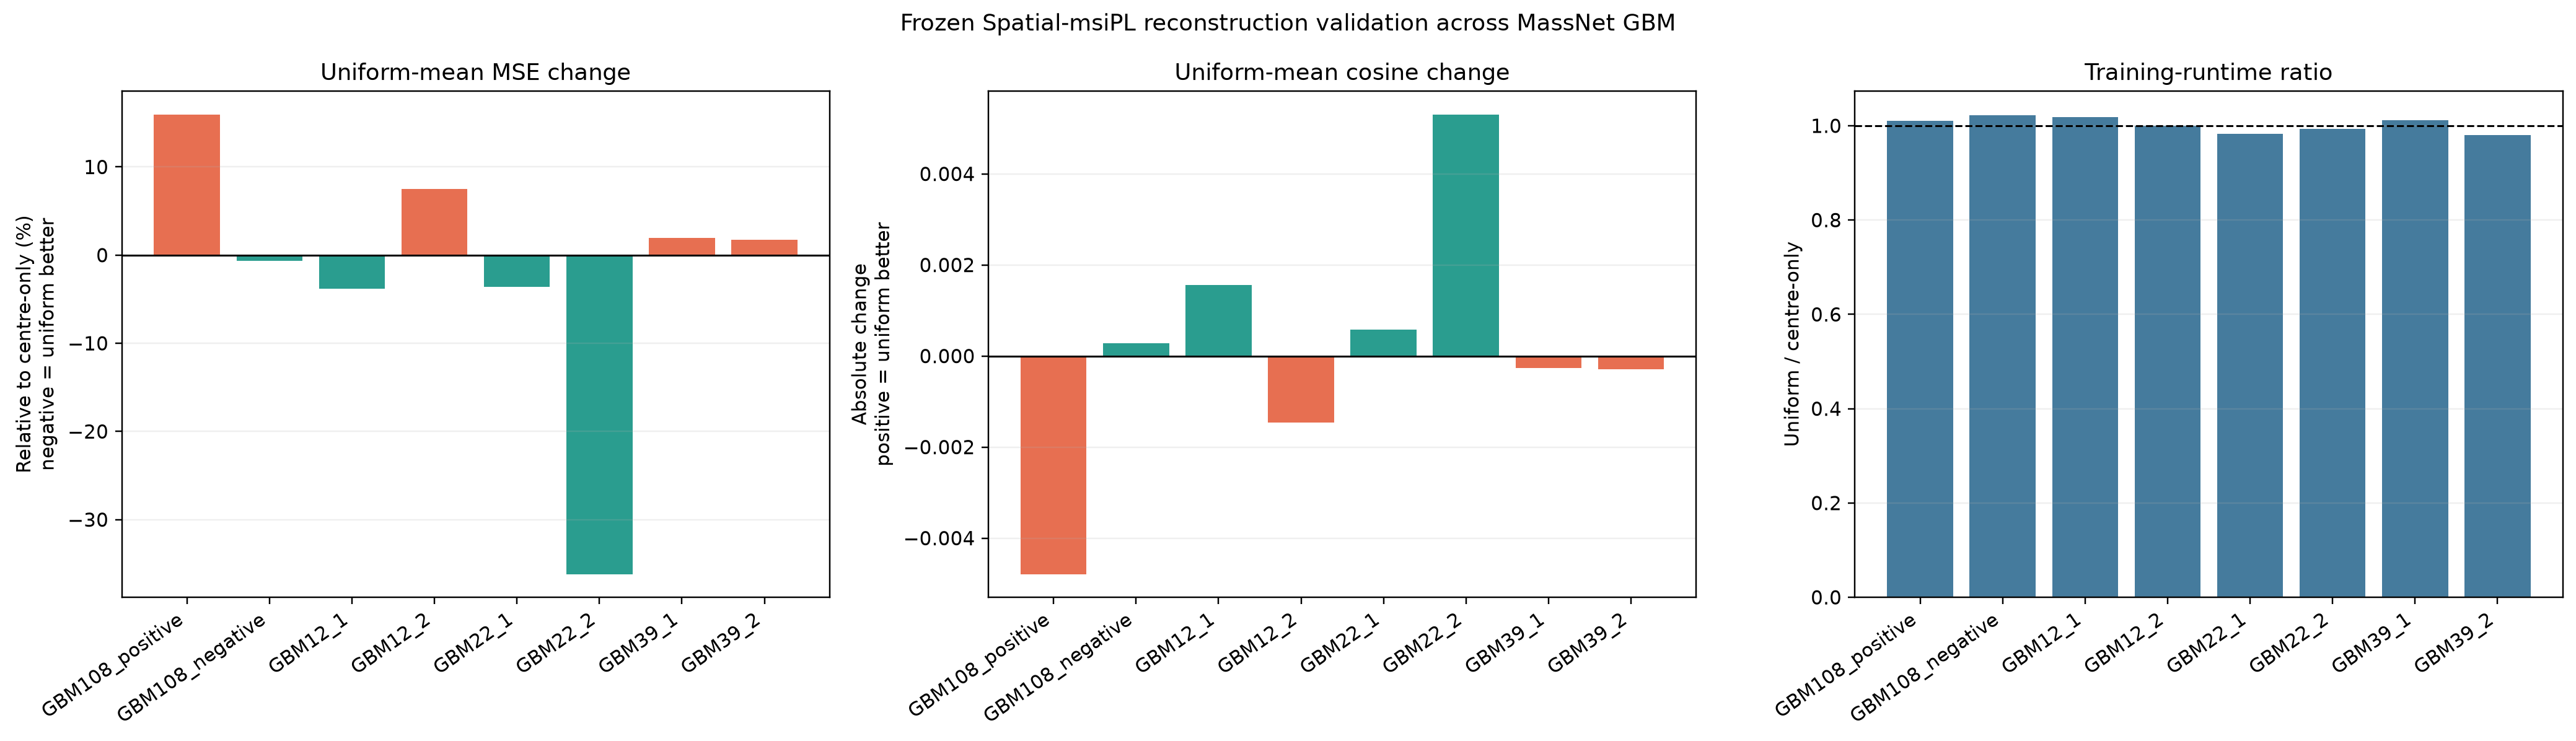
\includegraphics[width=\columnwidth]{images/gbm_reconstruction_validation.png}
  \caption{Paired whole-GBM reconstruction comparison. Negative MSE change
  favours uniform context; the heterogeneous section effects produce no
  consistent aggregate advantage.}
  \label{fig:recon}
\end{figure}

The peak-selection effect was also collection-dependent
(\Cref{fig:context}). On GBM, uniform-context IG averaged 0.4562 mSCF1 versus
0.4665 for centre-only IG, winning five of eight sections but with mean change
$-0.0103$. On CAC, it averaged 0.5595 versus 0.5285, won all eight sections and
had a mean paired gain of 0.0310 (exact $p=0.0078125$). Thus context changed the
nonlinear ranking beneficially on CAC without a corresponding universal gain
in reconstruction or GMM--mask agreement.

\begin{figure*}[t]
  \centering
  
\includegraphics[width=0.96\textwidth]{images/figure_2_context_effect_by_section.png}
  \caption{Section-wise change in mSCF1 from adding uniform neighbourhood
  context to the otherwise matched VAE and GMM-targeted IG procedure. Context
  is mixed on GBM but positive on every CAC section.}
  \label{fig:context}
\end{figure*}

\subsection{Does nonlinear attribution improve peak ranking?}

\Cref{fig:primary} summarises the primary matched-count result. On GBM,
centre-only IG and uniform-context IG averaged 0.4665 and 0.4562 mSCF1,
respectively, versus 0.3643 for legacy msiPL. At least one IG variant beat
legacy msiPL in every section; uniform-context IG alone did so in all eight
($p=0.0078125$). On CAC, centre-only and uniform-context IG averaged 0.5285 and
0.5595 versus 0.4024 for legacy msiPL; uniform-context IG again won all eight
paired sections ($p=0.0078125$).

\begin{figure*}[t]
  \centering
  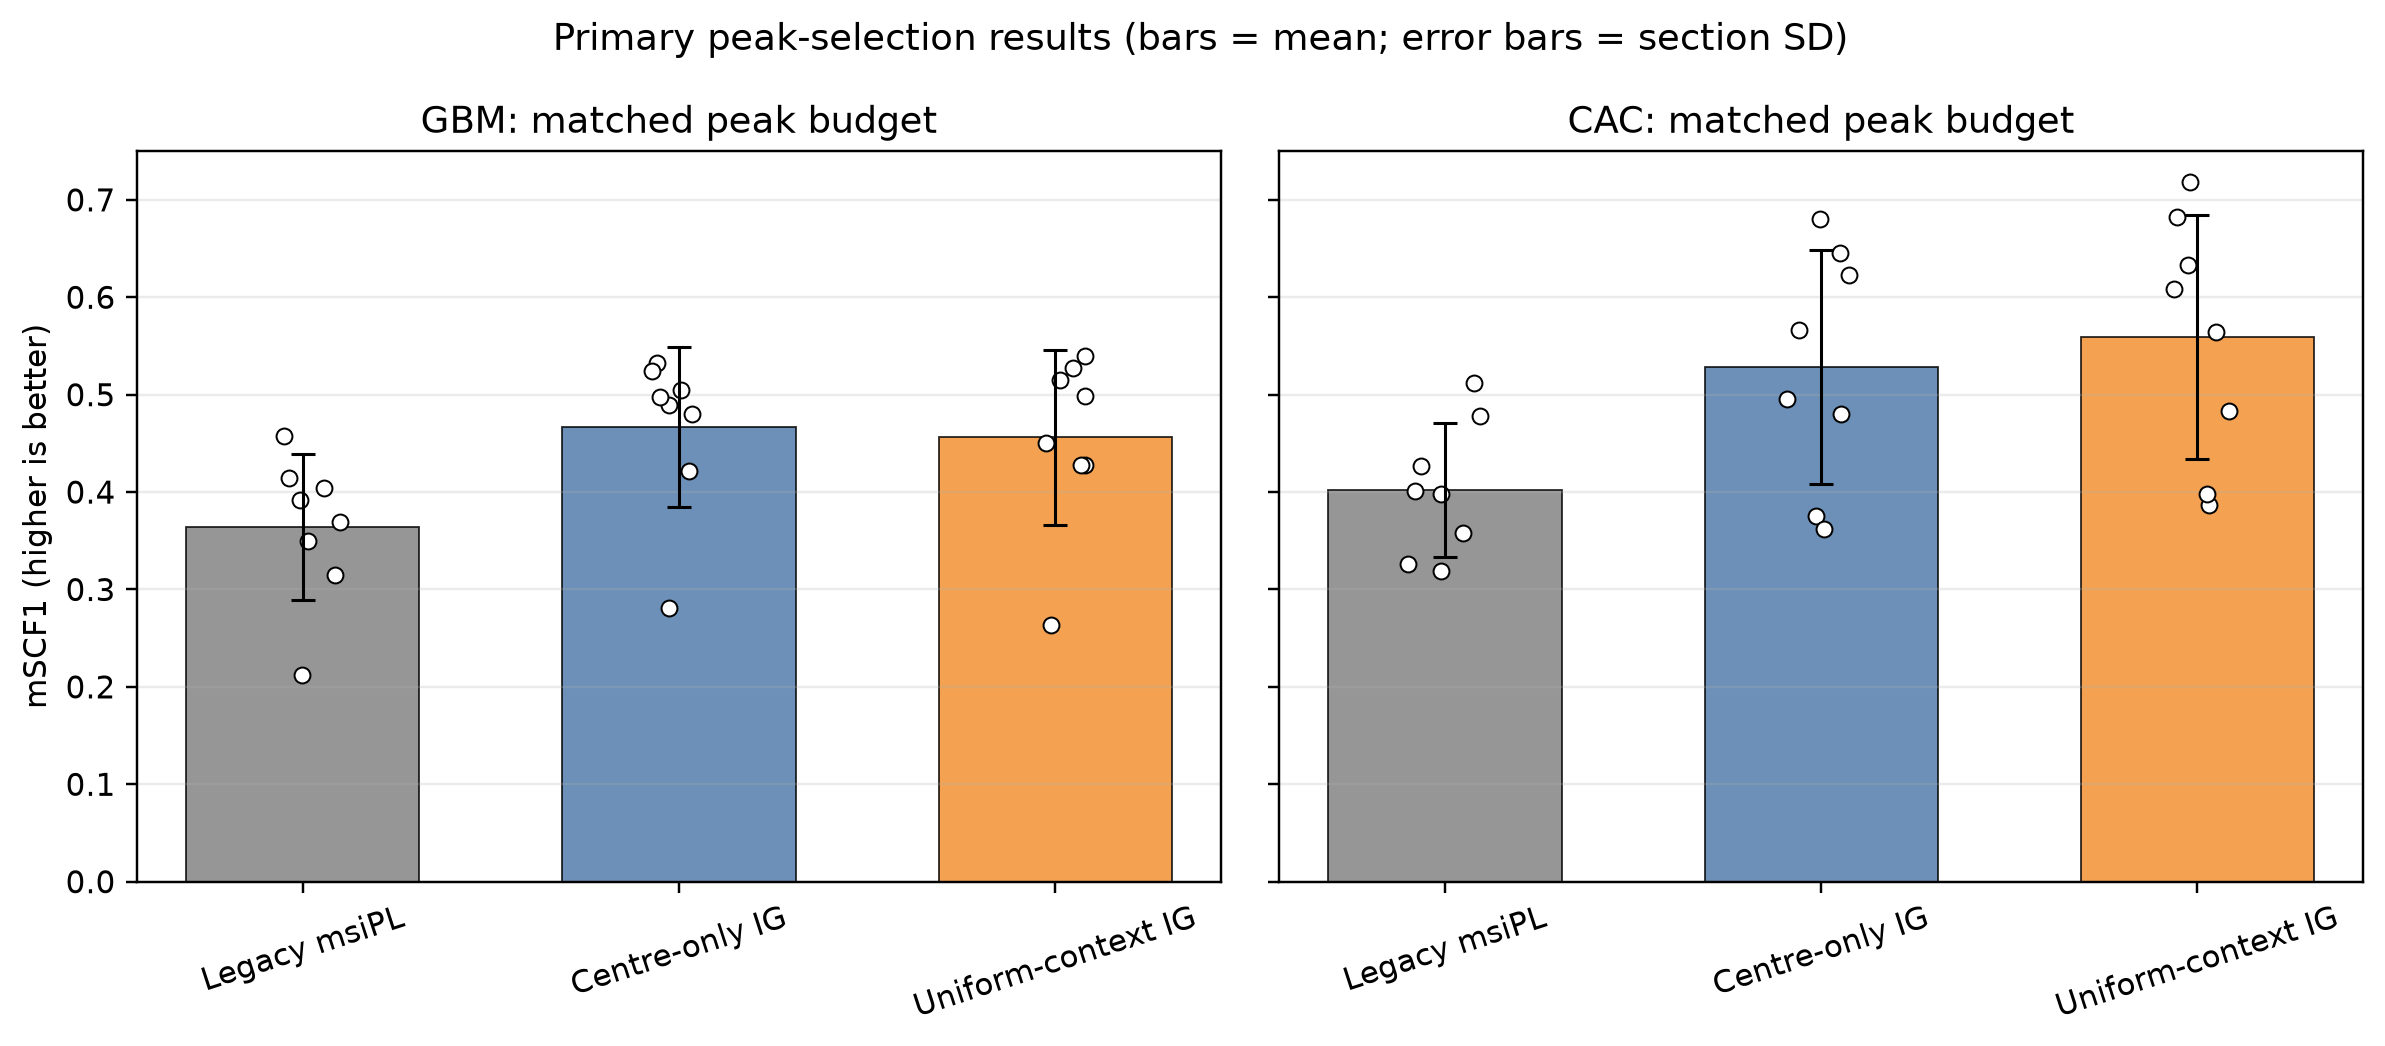
\includegraphics[width=0.96\textwidth]{images/figure_1_primary_peak_quality.png}
  \caption{Matched-count peak-selection quality across the two collections.
  Markers represent tissue sections; bars summarise method-level means. The
  consistent comparison is within collection and section, not between the two
  different datasets.}
  \label{fig:primary}
\end{figure*}

First-layer L2 was generally much weaker than nonlinear IG
(\Cref{fig:ablation}). On the initial GBM108-positive test at 530 peaks,
uniform-context IG achieved 0.528 mSCF1, legacy msiPL 0.404 and first-layer L2
0.068. IG passed the numerical completeness checks, and deleting IG-ranked
features caused a larger GMM-posterior drop than deleting L2-ranked or random
features. These results support the interpretation that gradients through the
complete nonlinear encoder and latent decision surface contain information that
is absent from the first layer alone.

\begin{figure}[t]
  \centering
  
\includegraphics[width=\columnwidth]{images/figure_3_explanation_ablation.png}
  \caption{Explanation-method ablation at matched peak counts. The simple
  first-layer L2 shortcut is not an adequate substitute for GMM-targeted
  nonlinear attribution.}
  \label{fig:ablation}
\end{figure}

S3PL remained stronger on matched CAC evaluation: 0.5915 versus 0.5595 for
uniform-context IG, winning six of eight sections (exact $p=0.0390625$). This
comparison establishes peak quality, but not equivalent computational
efficiency: S3PL used its released 10-epoch protocol whereas the VAE validation
used 100 epochs.

\subsection{Learned attention and training-seed stability}

Corrected attention, uniform mean and centre-only models were independently
trained with seeds 1--3 on the frozen GBM108-positive development section. Mean
mSCF1 was $0.5120\pm0.0179$, $0.5250\pm0.0132$ and
$0.5454\pm0.0188$ (sample standard deviation), respectively
(\Cref{fig:seeds}). Attention beat uniform mean in all three paired seeds, with
gains $+0.0347$, $+0.0120$ and $+0.0144$ (mean $+0.0204$). Mean GMM balanced
accuracy was 0.8745, 0.8735 and 0.8822.

\begin{figure*}[t]
  \centering
  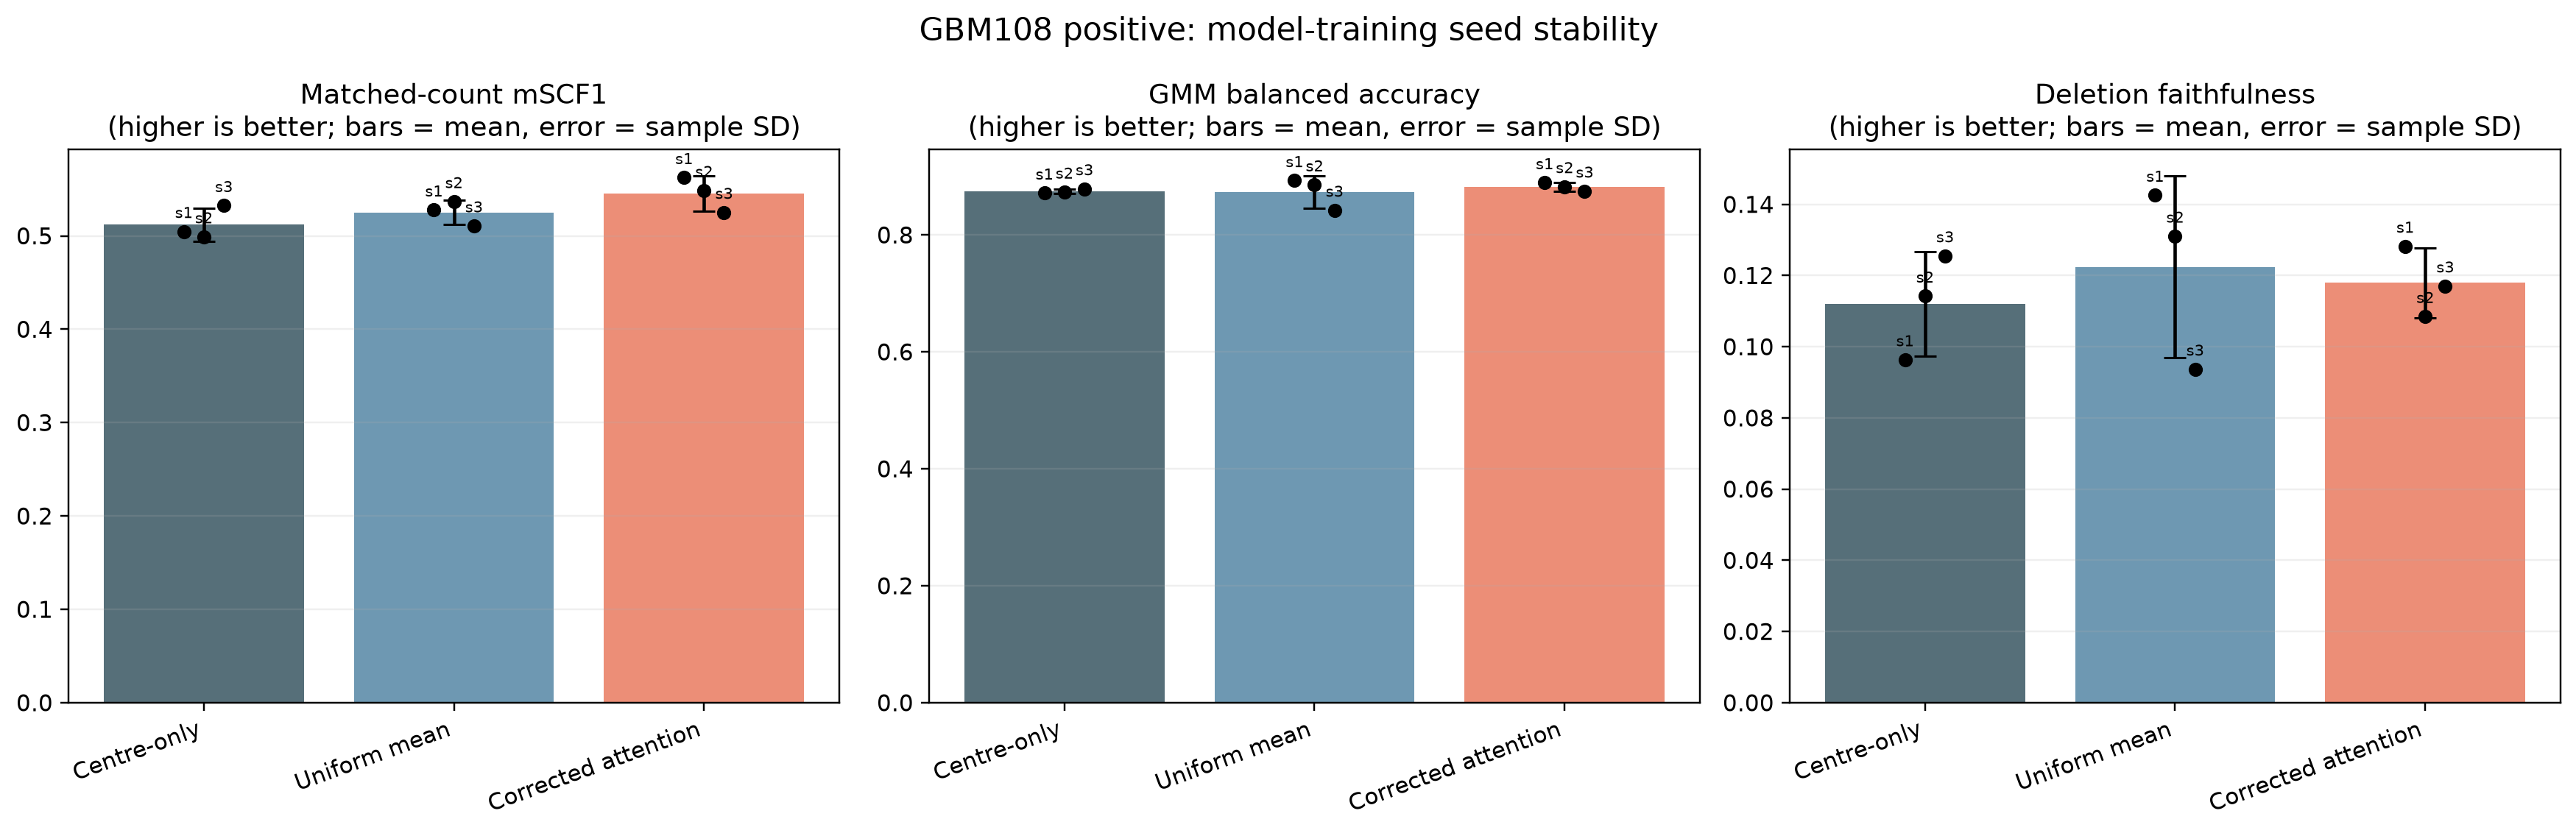
\includegraphics[width=0.95\textwidth]{images/figure_4_seed_stability.png}
  \caption{Targeted three-seed stability on GBM108-positive. Corrected
  attention improves matched-count mSCF1 over uniform averaging in every seed,
  but the experiment is restricted to one development section.}
  \label{fig:seeds}
\end{figure*}

The attention result did not pass the combined predeclared gate. Its mean
deletion-faithfulness score was 0.0045 below uniform mean and it won that metric
in only one seed. Peak allocated GPU memory also increased from about 2.90 GiB
for uniform mean to 3.20 GiB for attention. The result is therefore a stable
peak-quality improvement on one section, not evidence of a uniformly superior
model.

\section{Discussion}
\label{sec:discussion}

The clearest result is not that spatial input always improves a VAE. It is that
the way a learned representation is explained matters strongly for peak
selection. Both centre-only and contextual GMM-targeted IG exceeded legacy
msiPL across the complete GBM and CAC evaluations, while first-layer L2 often
failed. This is consistent with the methodological difference: L2 observes one
linear transformation, whereas IG follows the full nonlinear path to a
label-free latent-space decision.

RQ1 has a conditional answer. Uniform context did not consistently improve GBM
reconstruction or mSCF1, but improved CAC mSCF1 in every paired section. A
neighbour mean can reduce local noise when adjacent spectra share relevant
structure, but can also blur boundaries or combine heterogeneous tissue. The
different spectral resolution, tissue classes, coverage and acquisition
properties of GBM and CAC plausibly change that balance. The experiments show
the boundary of the effect; they do not identify one biological cause.

RQ2 is supported more broadly. Nonlinear IG improved matched-count peak quality
over legacy msiPL across both collections. Completeness and deletion tests add
important evidence beyond mSCF1: the former checks numerical consistency with
the explained output, while the latter asks whether removing highly ranked bins
actually changes that output. Nevertheless, a high mask-correlation score does
not validate a peak as a biomarker. Independent molecular identification and
biological validation remain outside this study.

RQ3 shows a trade-off. Corrected attention gave a small but seed-consistent
mSCF1 improvement on the development section, yet did not improve deletion
faithfulness and consumed more memory. It should therefore remain an ablation
until tested across independent sections. Uniform averaging remains the more
defensible broad-validation model because it is parameter-free and was frozen
before whole-dataset evaluation.

S3PL is the strongest executable CAC baseline in peak quality. The present
method should not be described as both more accurate and cheaper than S3PL: its
matched CAC mSCF1 is lower, and the 10- versus 100-epoch protocols make the
recorded runtimes non-equivalent. The value of Spatial-msiPL is instead the
controlled evidence about context and attribution within a VAE framework.

Limitations include seed-1 section-wide validation, three-seed testing on only
one development section, sections that are not independent patients,
dataset-specific peak budgets, a GBM S3PL reproduction gap, and variable
cluster hardware availability. Future work should repeat training across
patients and sections, constrain attention more efficiently, investigate
automatic peak-budget selection, and validate selected ions biologically.

\section{Conclusion}
\label{sec:conclusion}

This study separated neighbourhood input from nonlinear peak attribution in a
lightweight MSI VAE. For RQ1, uniform eight-neighbour context was not a
universal improvement: GBM reconstruction and mSCF1 were mixed, while CAC
mSCF1 improved in all eight sections. For RQ2, label-free GMM-targeted
Integrated Gradients was the robust contribution, improving matched-count peak
quality over legacy msiPL throughout both collections and substantially
outperforming simple first-layer L2 importance. For RQ3, corrected attention
improved mSCF1 over uniform averaging across three training seeds on one
development section, but its faithfulness and memory trade-offs prevented its
promotion as the final general method. S3PL remained stronger on matched CAC
peak quality. The resulting conclusion is deliberately bounded: nonlinear
attribution makes the VAE representation more useful for peak ranking, whereas
the value of spatial context depends on the dataset and aggregation mechanism.


\section*{Acknowledgements}
The author thanks Hairong Bau and Richard Klein for their supervision and
guidance, and the University of the Witwatersrand for access to the MSCluster
computing facility.

\balance
\bibliography{references}
\end{document}
